\documentclass[a4paper]{article}

%% Language and font encodings
\usepackage[english]{babel}
\usepackage[utf8x]{inputenc}
\usepackage[T1]{fontenc}
\usepackage{makecell}

%% Sets page size and margins
\usepackage[a4paper,top=3cm,bottom=2cm,left=3cm,right=3cm,marginparwidth=1.75cm]{geometry}

%% Useful packages
\usepackage{amsmath}
\usepackage{amssymb}
\usepackage{amsfonts}
\usepackage[shortlabels]{enumitem}
\usepackage{graphicx}
\usepackage{tikz}
\usetikzlibrary{arrows.meta}
\newcommand\independent{\perp \!\!\! \perp}

%% display solutions or not
\newif\ifsol
% \soltrue % comment out to hide solutions

\usepackage[colorinlistoftodos]{todonotes}
\usepackage[colorlinks=true, allcolors=blue]{hyperref}

\usepackage{color}
\usepackage{url}

\title{Exam 2 - Practice Problems}
\author{CS 182 - Artificial Intelligence}
\date{}

\begin{document}
\maketitle

Note: we have pulled many of these problems from previous Berkeley exams which can be found at: \href{http://ai.berkeley.edu/exams.html}{\texttt{http://ai.berkeley.edu/exams.html}}. We cannot promise that all of those exams cover relevant material but will note that there are additional questions of these types that are applicable for certain parts of this review.

\section{Robot Motion Planning}
    \noindent \textbf{Problem 1:} We have a two link robotic arm with rotational joints one fixed at (0,0) and the other fixed to the end of the first link. Both links are $3\sqrt{2}$ meters long and the 0 angle is defined by the dashed line in the left side of the picture below (from the x-axis for $\theta_1$ and aligned with the first link for $\theta_2$. There is one obstacle, the large red polygon. We have decided to build a PRM to plan collision free paths (where a collision is defined as any part of the robot touching an obstacle). We samples 5 points in configuration space labeled a to e in the configuration space diagram on the right side of the picture below. Which points can we keep as milestone for our PRM? \\ \textit{Hint: $45^o$ = $\frac{\pi}{4}$ radians and 45-45-90 triangles have side lengths 1-1-$\sqrt{2}$)}\\
    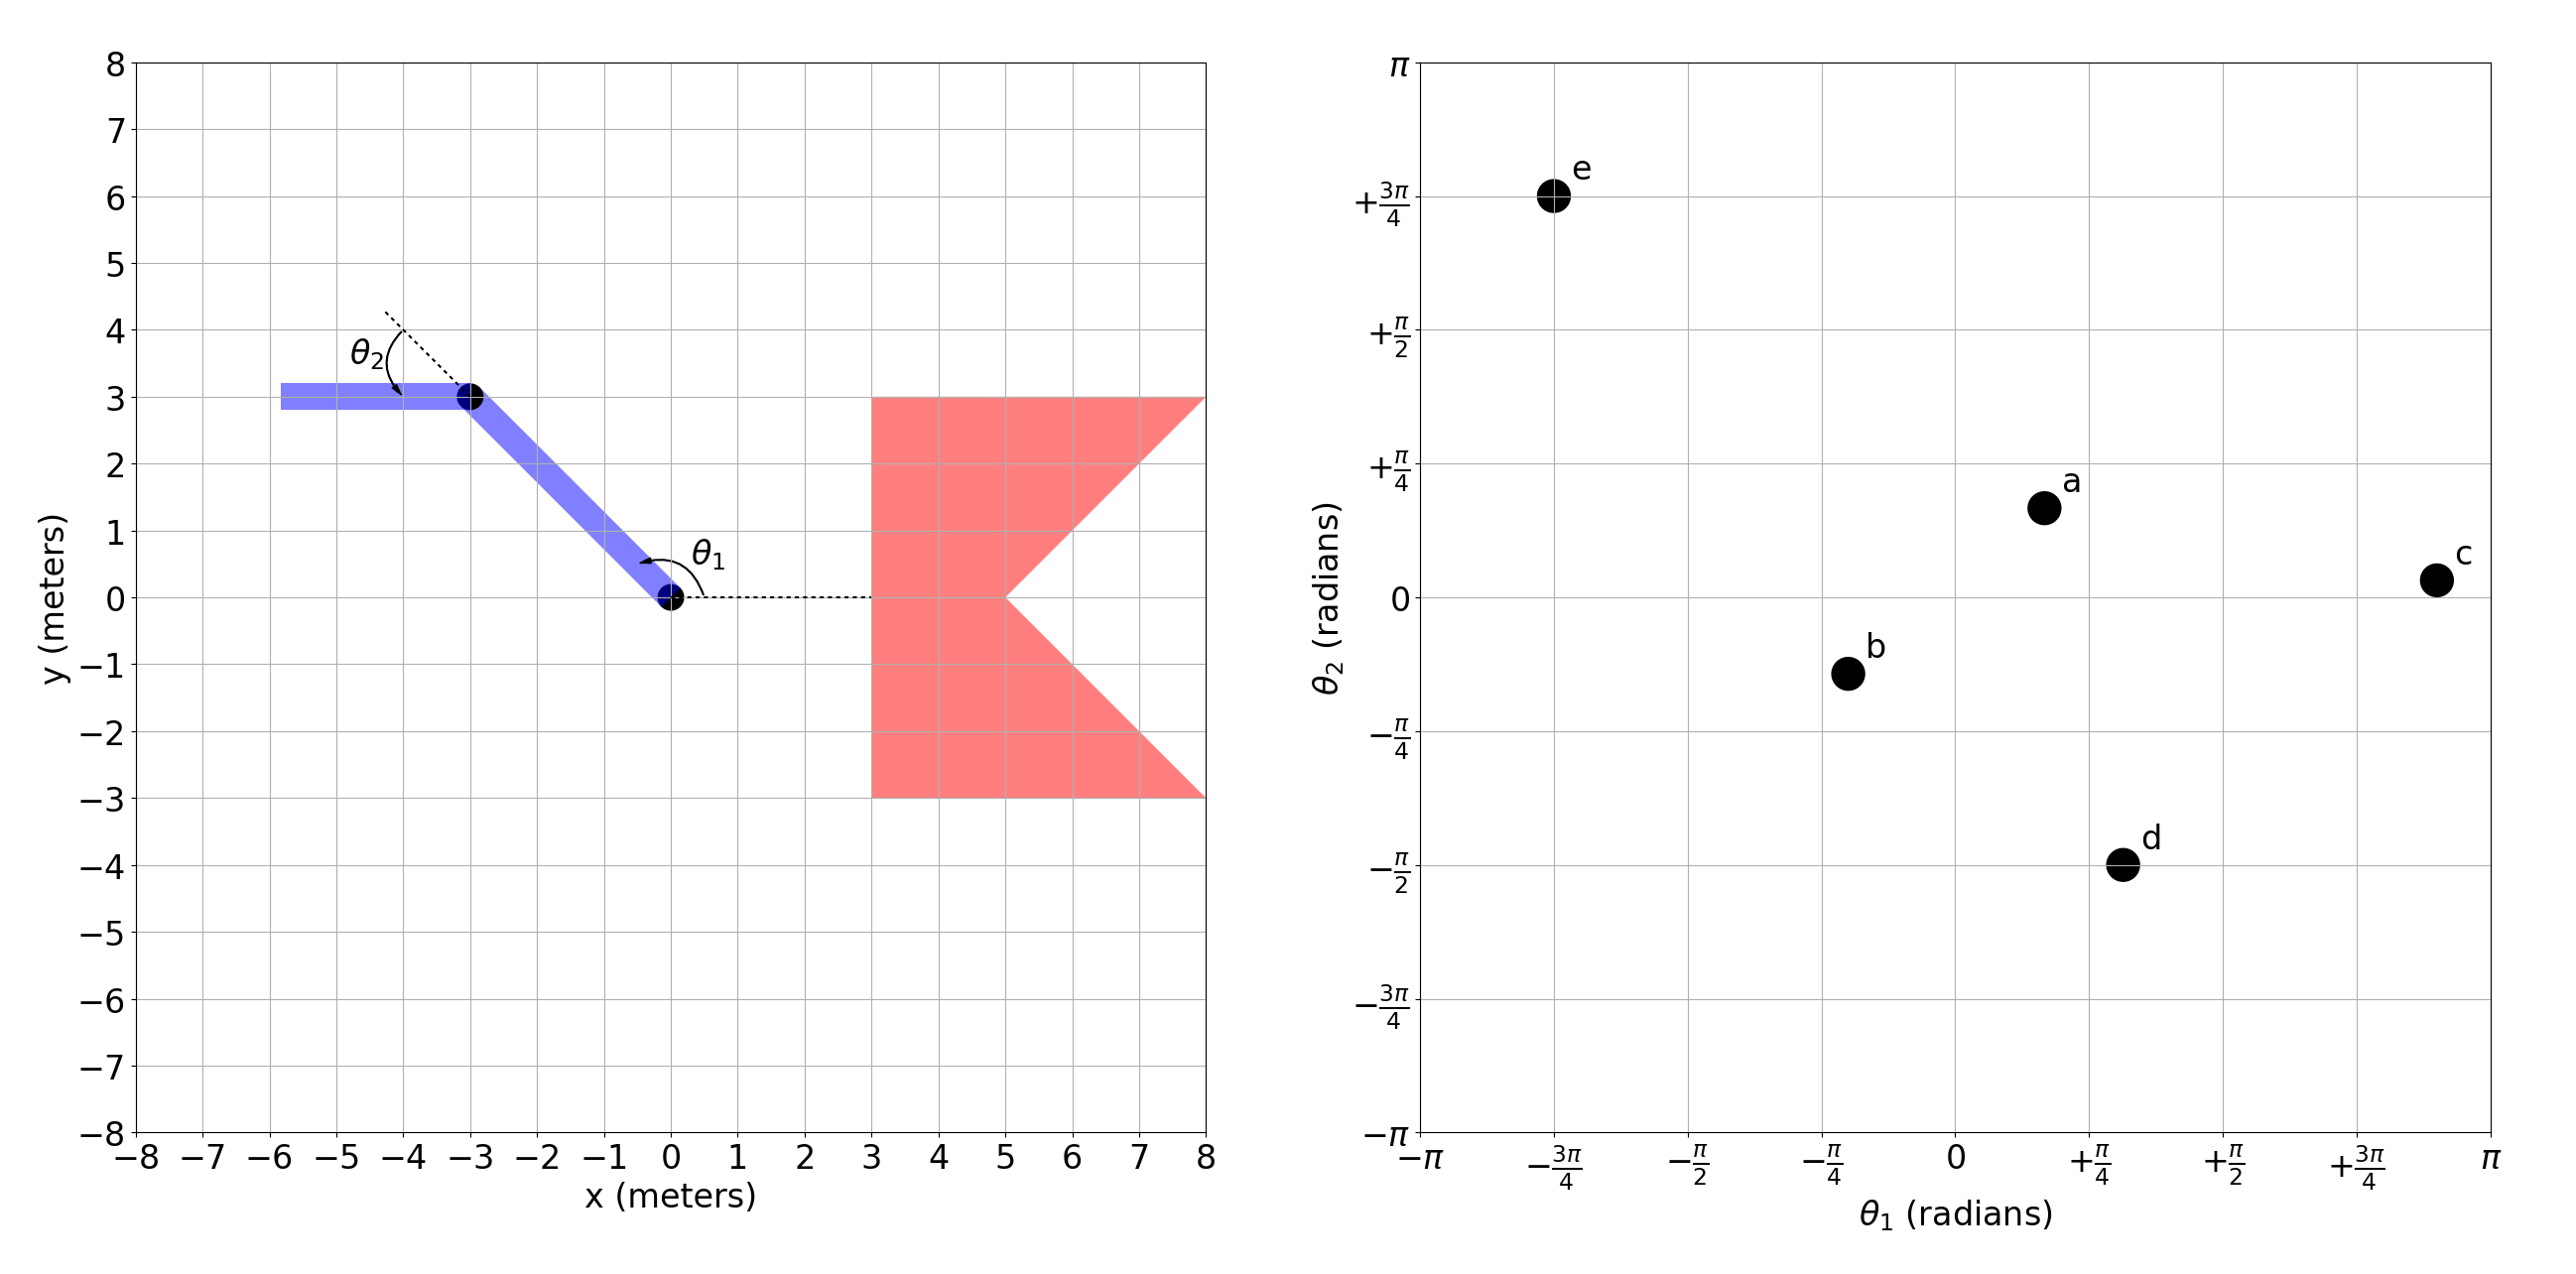
\includegraphics[width=\textwidth]{figs/multiPoint.png}\\
    \ifsol {\color{blue} We can retain only the collision free samples. We can note that since the ``elbow'' of the robot will be in collision when $-\frac{\pi}{4} < \theta_1 < \frac{\pi}{4}$ we can discard samples a and b. We can also discard sample d as while the first link will just be outside the obstacle the second link will be turned down and hitting the obstacle. Samples c and e have the arm on the left side of the task space and thus safe and can be kept for the PRM.}
    \bigskip
    \else \bigskip \bigskip \bigskip \bigskip \bigskip
    \fi
    
    \noindent \textbf{Problem 2:} When would you consider using trajectory optimization over RRT?\\
    \ifsol {\color{blue} Some potential answers would include: \begin{itemize}
        \item When a robot is moving fast and the dynamics matter (and it has complex dynamics)
        \item When we want a locally optimal trajectory and not just a feasible trajectory
        \item When it is easier to come up with a relevant cost function than a relevant distance metric
    \end{itemize}}
    \bigskip
    \else \bigskip \bigskip \bigskip \bigskip
    \fi
    
    \newpage
    \noindent \textbf{Problem 3:} Consider the AdaptiveStep-RRT (AS-RRT) algorithm (the blue lines indicate additional steps taken in AS-RRT compared to standard RRT):
    \begin{itemize}
		\item Algorithm AS-RRT (input: start state $s_0$, goal $s_G$, initial tree $T = s_0$, {\color{blue} max extend distance $d_{max}$, min extend distance $d_{min}$, step size change $\delta$})
		\item \quad For $i=1,\dots, N$:
		\item \quad \quad Sample states $s \in \mathcal{S}$ until $s$ is collision-free
		\item \quad \quad Find closest state $s_c \in T$
		\item \quad \quad {\color{blue}Set $d = d_{max}$}
		\item \quad \quad {\color{blue}While($d > d_{min}$):}
		\item \quad \quad \quad Extend $s_c$ toward $s$ with distance $d$ resulting in state $s'$
		\item \quad \quad \quad If isCollisionFreePath($s_c$, $s'$):
		\item \quad \quad \quad \quad Add $s'$ to $T$
		\item \quad \quad \quad \quad {\color{blue}Break}
		\item \quad \quad \quad {\color{blue}{Else:}}
		\item \quad \quad \quad \quad $d = d - \delta$
		\item \quad Return $T$
	\end{itemize}\\
	\begin{enumerate}[a)]
	    \item Assume that we are using a k-d tree where insert and nearest searches take $O(log|T|)$ and that sample, extend, and isCollisionFreePath are $O(1)$ operations, what is the worst case time coplexity for one iteration of AdaptiveStep-RRT? \\ \\
	    \ifsol {\color{blue} On each iteration we perform 1 sample, 1 closest state search, 1 insertion, and $O(\frac{d_{max}-d_{min}}{\delta})$ extends and collision checks. Therefore our total complexity is $O\left( \frac{d_{max}-d_{min}}{\delta} + log(|T|)\right)$.}
	    \bigskip
	    \else \bigskip \bigskip \bigskip \bigskip
	    \fi
	    
	    \item Do you think that the assumption that isCollisionFreePath is always an $O(1)$ operation is reasonable? Why or why not? \\ \\
	    \ifsol {\color{blue} No because for large values of $d$ we will need to check many points along the path for collisions in order to ensure that our solution is collision free. In fact due to this issue in practice the algorithm is often implemented in one of two ways: \begin{enumerate}
	        \item Instead of simply doing $d = d - \delta$, $d$ is set to a value just smaller than the distance to the first computed collision. In order to attempt to greedily converge in two iterations. Of course depending on how the collision checker is implemented, the first collision found may or may not be the farthest one along the path, and some collision checkers do not return the location of the collision just its existence.
	        \item Alternatively, the algorithm starts with $d = d_{min}$ and adds $\delta$ until it has its first collision, ensuring on each iteration that one only needs to check for collisions in the $|\delta|$ additional extension.
	    \end{enumerate}}
	    \bigskip
	    \else \bigskip \bigskip \bigskip \bigskip
	    \fi
	\end{enumerate}\\
%%%%%%%%%%%%%%%%%%%%%%%%%%%%%%%%%%%%%%%%%%%%%%%%%%%%%%%%%%%%%%%%%%%%%%%%%
%%%%%%%%%%%%%%%%%%%%%%%%%%%%%%%%%%%%%%%%%%%%%%%%%%%%%%%%%%%%%%%%%%%%%%%%%
\newpage
\section{Probability Review}
    Note: I wouldn't expect a question dedicated to this on the exam but you need to be comfortable with joint vs. marginal vs. conditional probabilites and how to move between them when working with HMMs and Bayes' Nets.\\
    \ifsol
        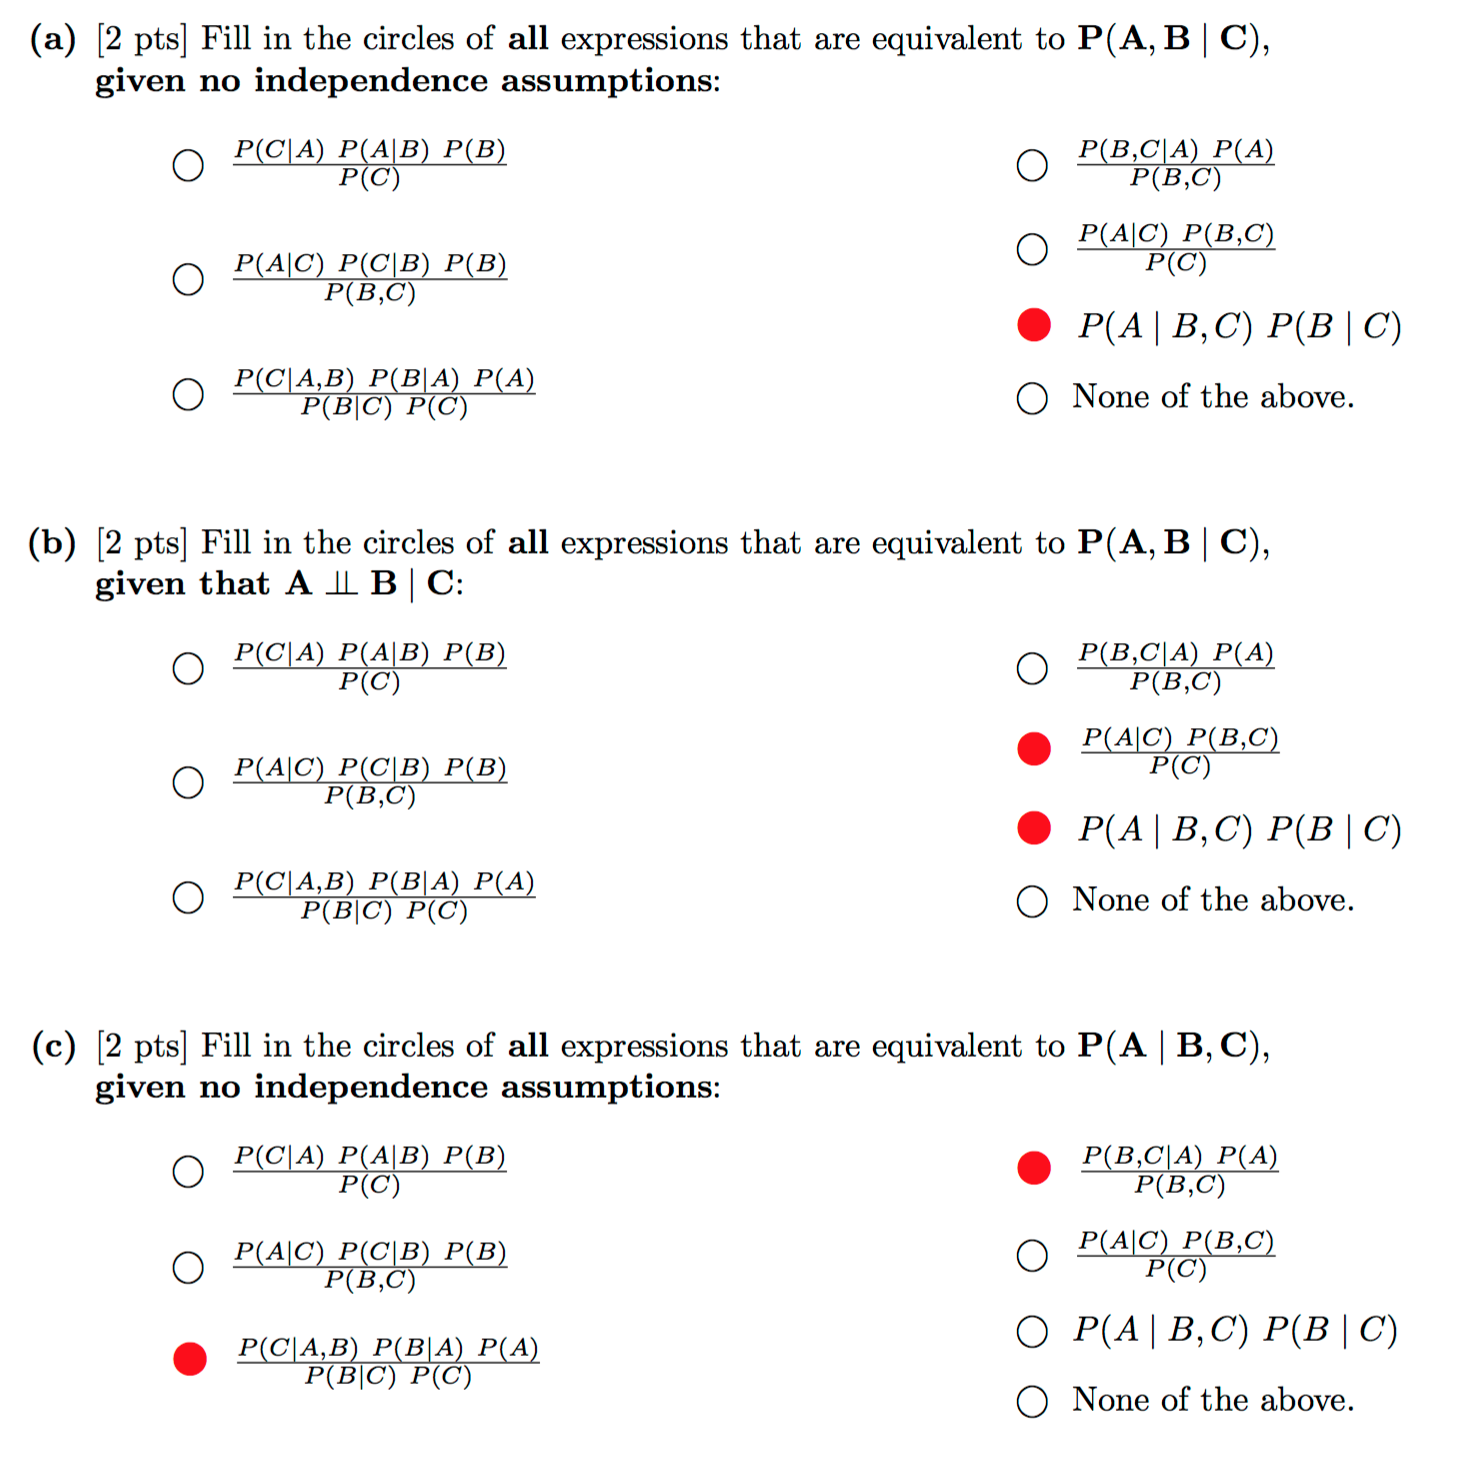
\includegraphics[width=\textwidth]{figs/probabilitysolutions.png}
    \else
        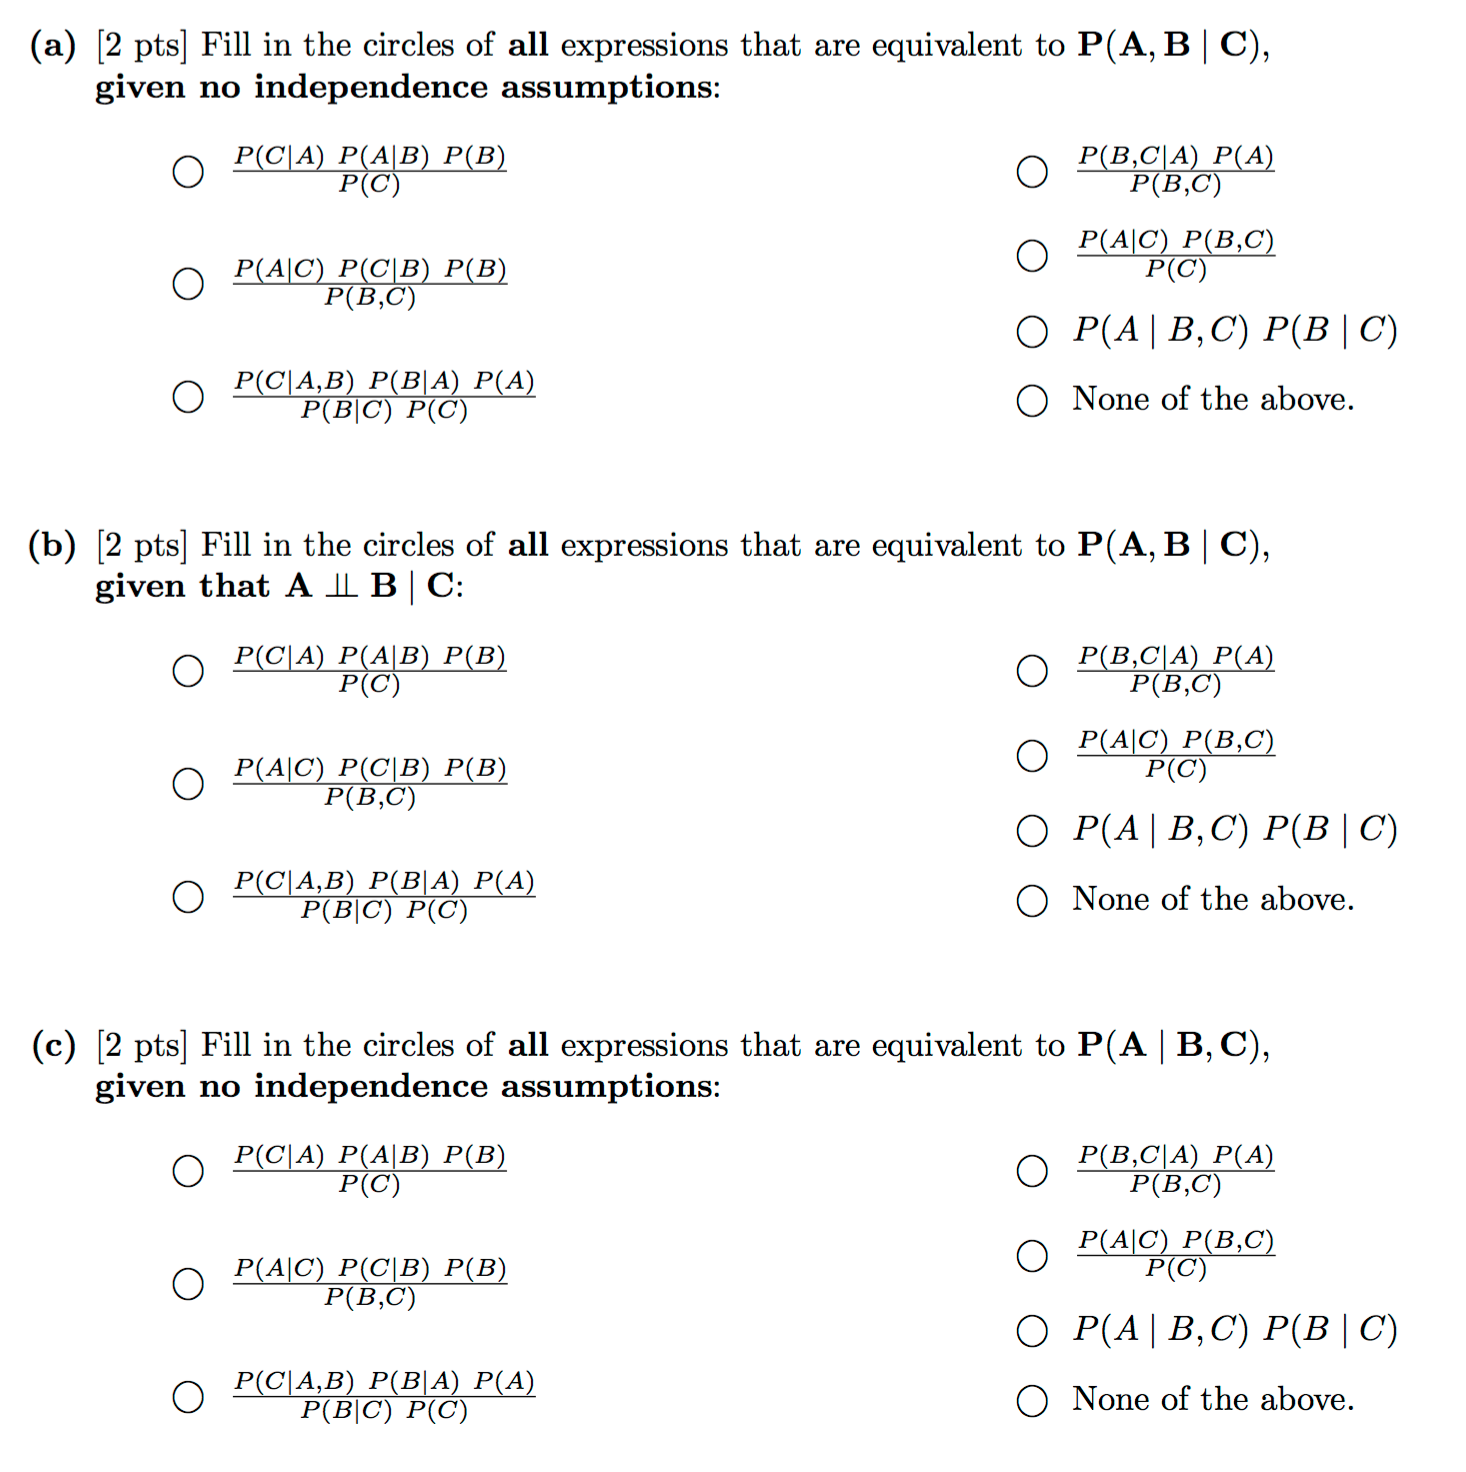
\includegraphics[width=\textwidth]{figs/probability.png}
    \fi
%%%%%%%%%%%%%%%%%%%%%%%%%%%%%%%%%%%%%%%%%%%%%%%%%%%%%%%%%%%%%%%%%%%%%%%%%
%%%%%%%%%%%%%%%%%%%%%%%%%%%%%%%%%%%%%%%%%%%%%%%%%%%%%%%%%%%%%%%%%%%%%%%%%
\newpage
\section{HMMs}
    \textbf{Problem 1:} Transportation researchers are trying to improve traffic in the city but, in order to do that, they first need to estimate the location of each of the cars in the city. They need our help to model this problem as an inference problem of an HMM. For this question, assume that only one car is being modeled.\\
    \begin{enumerate}[a)]
        \item The structure of this modified HMM is given below, which includes $X$, the location of the car; $S$, the noisy location of the car from the signal strength at a nearby cell phone tower; and $G$, the noisy location of the car from GPS.\\
        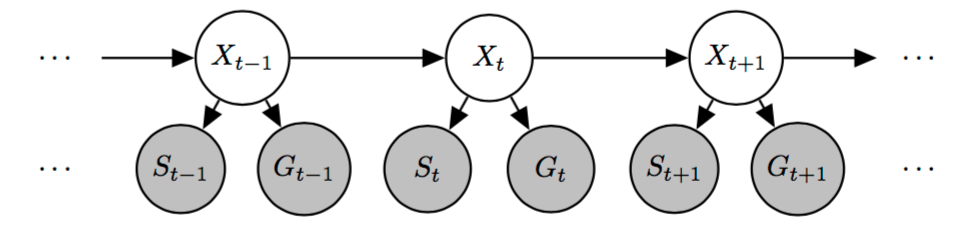
\includegraphics[scale=0.5]{figs/hmm.png}\\
        \ifsol
            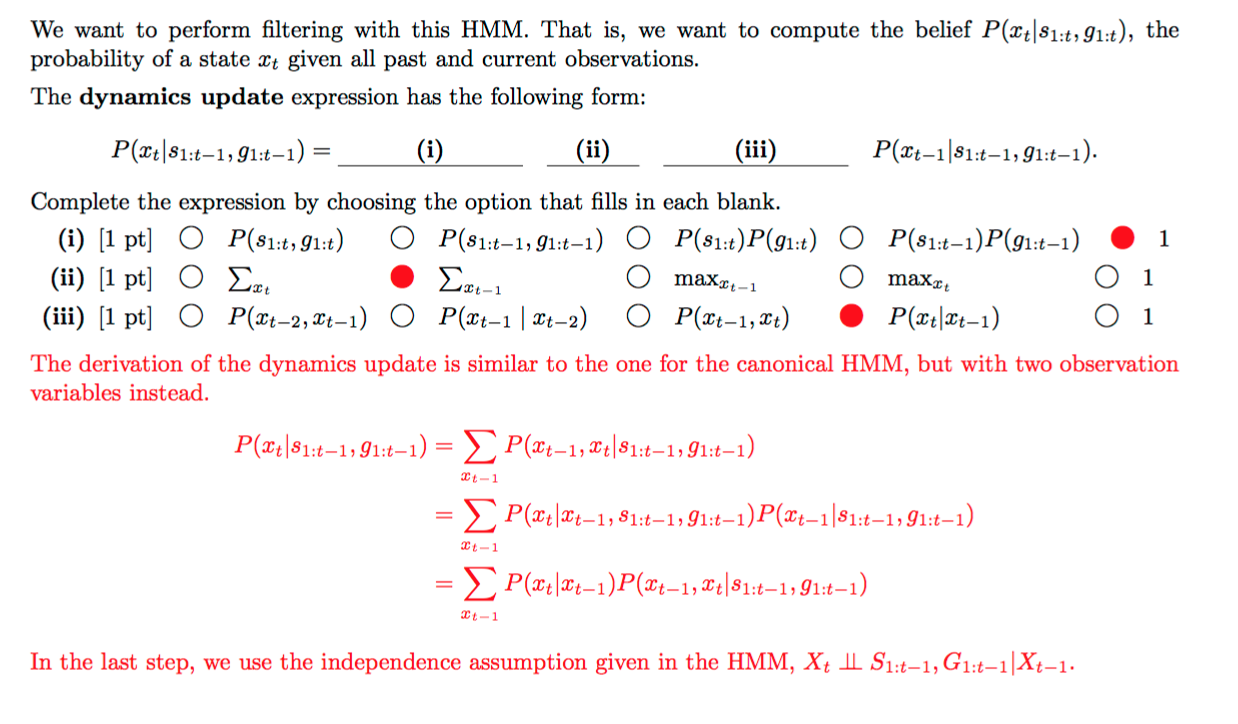
\includegraphics[scale=0.58]{figs/dynamicssolution.png}\\
            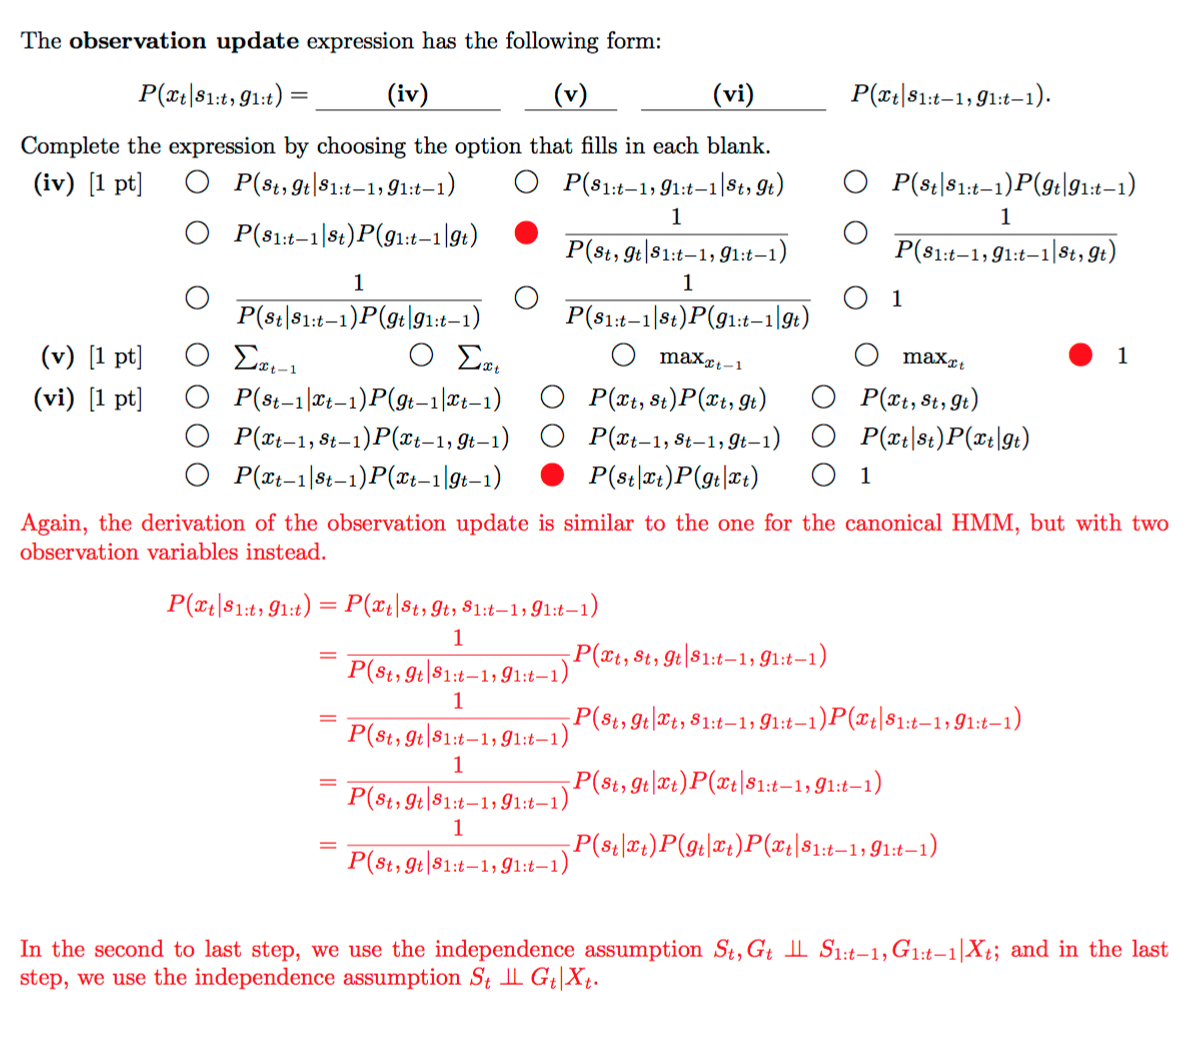
\includegraphics[scale=0.58]{figs/observationsolution.png}
        \else
            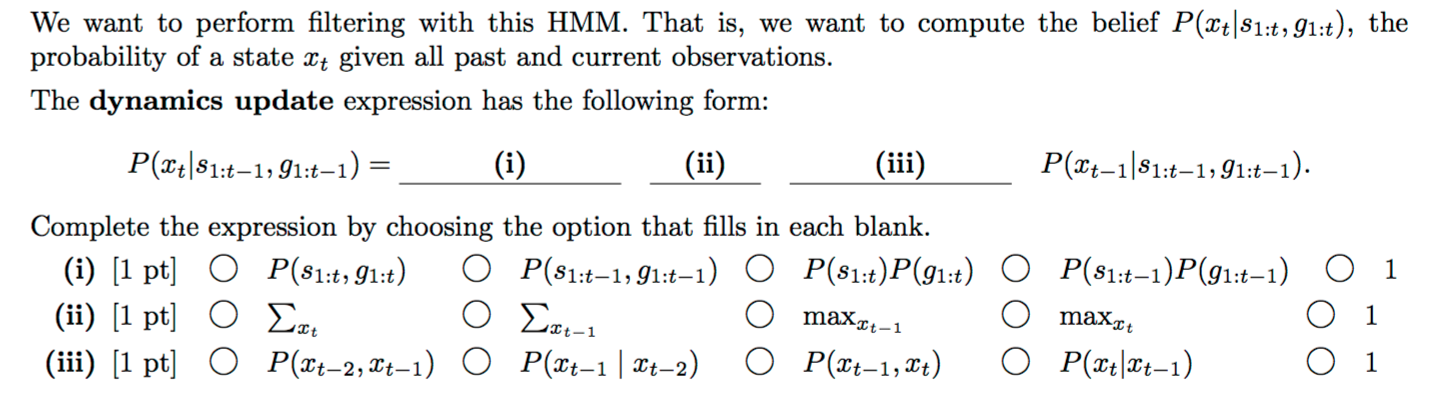
\includegraphics[scale=0.55]{figs/dynamics.png}\\
            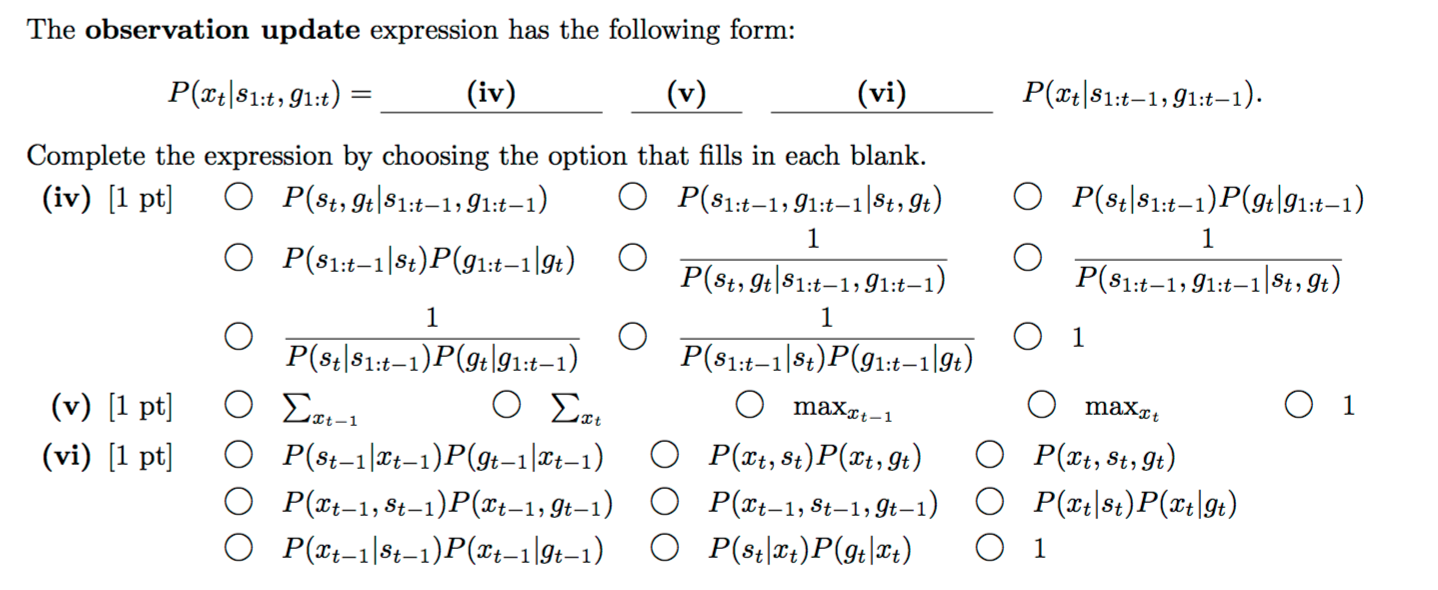
\includegraphics[scale=0.55]{figs/observation.png}
        \fi
        \item It turns out that if the car moves too fast, the quality of the cell phone signal decreases. Thus, the signal-dependent location $S_t$ not only depends on the current state $X_t$ but it also depends on the previous state $X_{t−1}$. Thus, we modify our original HMM for a new more accurate one, which is given below. Again, we want to compute the belief $P(xt|s_{1:t},g_{1:t})$. In this part we consider an update that combines the dynamics and observation update in a single update.\\
        \ifsol
            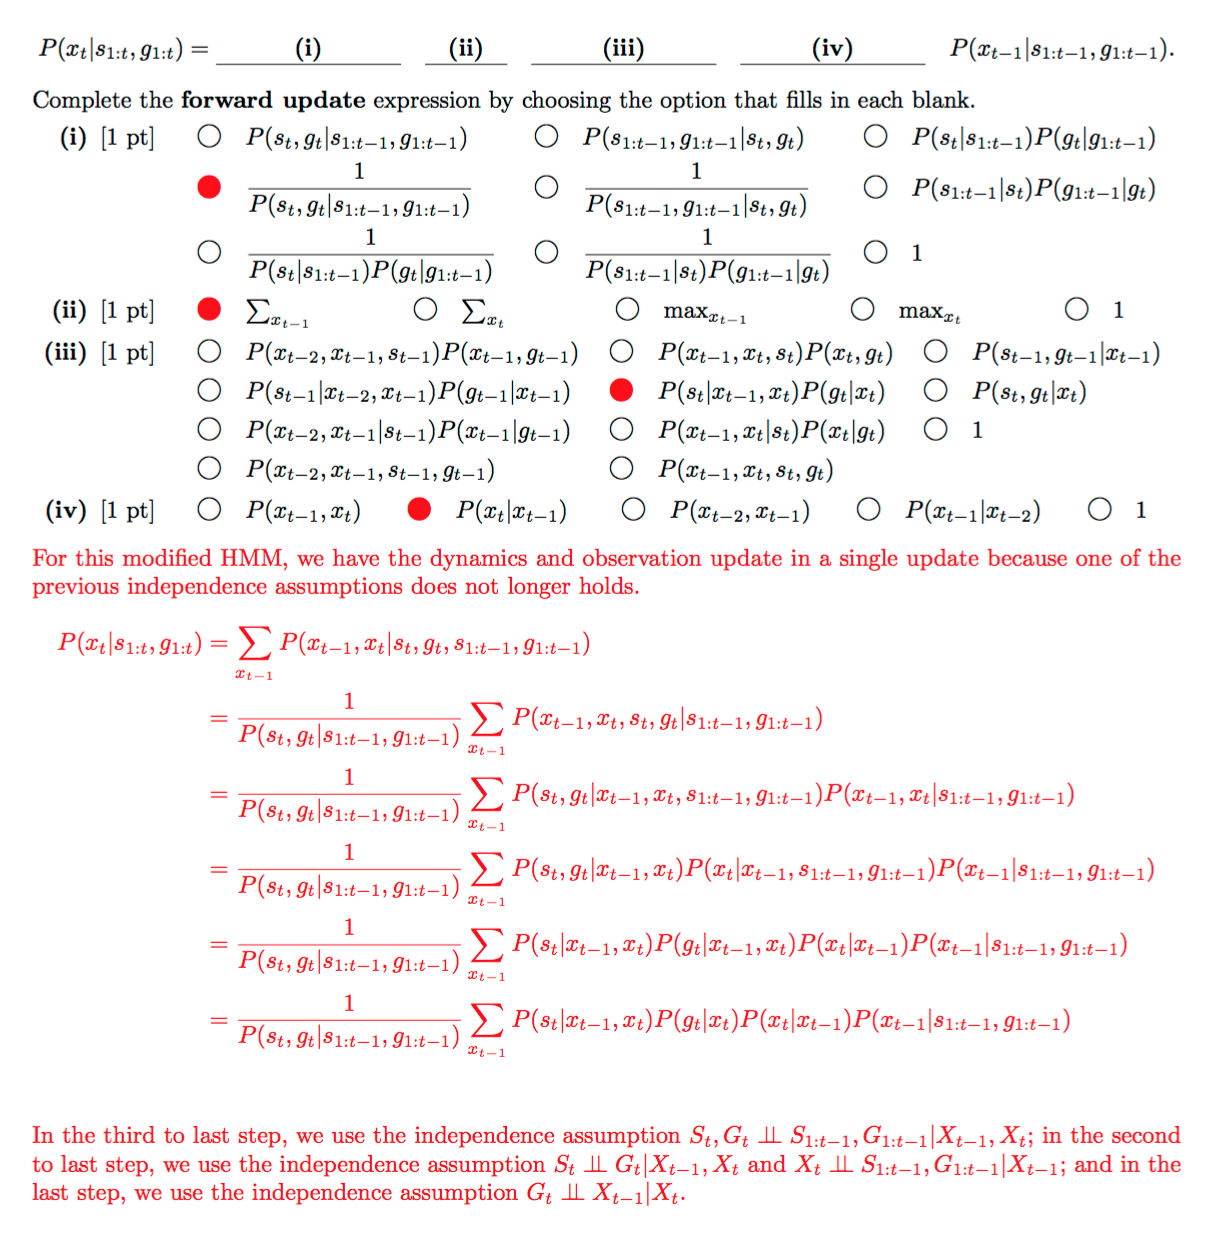
\includegraphics[scale=0.55]{figs/forwardsolution.png}
        \else
            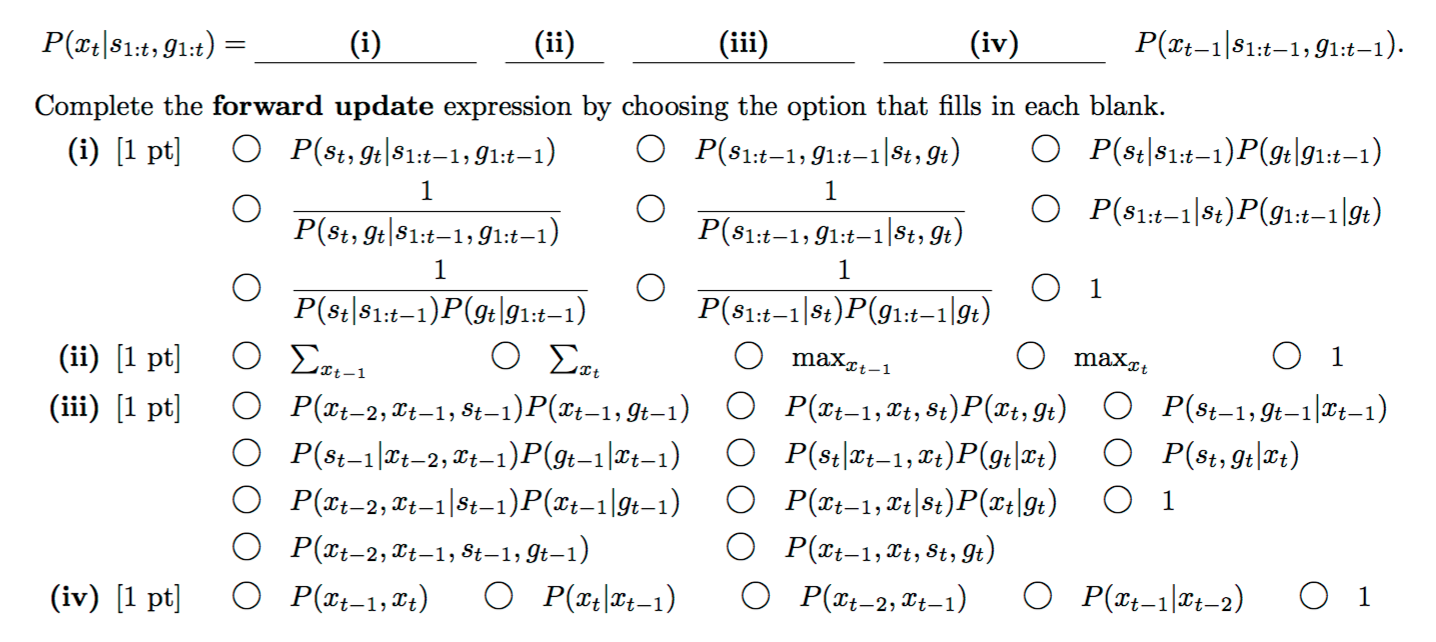
\includegraphics[scale=0.5]{figs/forward.png}
        \fi
    \end{enumerate}
    
    \noindent \textbf{Problem 2:} Pacman is trying to hunt a ghost in an infinite hallway with positions labeled as in the picture below. He’s become more technologically savvy, and decided to locate find the ghosts actual position, $S_t$, using some sensors he set up. From the sensors, Pacman can find, at each time step, a noisy reading of the ghost’s location, $O_t$. However, just as Pacman has gained technology, so has the ghost. It is able to cloak itself at each time step, given by $C_t$, adding extra noise to Pacman’s sensor readings.\\
    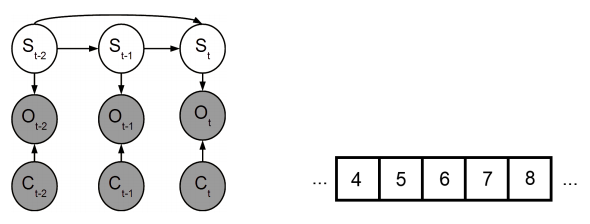
\includegraphics[scale=0.55]{figs/pacparticleprobhmm.png}\\
    Pacman has generated an error model, given in the table below, for the sensor depending on whether the ghost is cloaked or not. Pacman has also generated a dynamics model, given in the table below, that takes into account the position of the ghost at the two previous timesteps.\\
    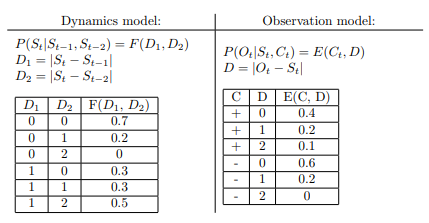
\includegraphics[scale=0.5]{figs/pacparticleprobmodels.png}\\
    \begin{enumerate}[a)]
        \item Assume that you currently have the following two particles: $(S_6 = 7, S_7 = 8)$ and $(S_6 = 6, S_7 = 6)$. Compute the weights for each particle given the observations: $$C_6 = +, C_7 = −, O_6 = 5, O_7 = 8$$
        \ifsol {\color{blue} 
        $(S_6 = 7, S_7 = 8)$: $P(O_6 = 5|C_6 = +, S_6 = 7) ∗ P(O_7 = 8|C_7 = −, S_7 = 8) = 0.1 ∗ 0.6 = 0.06$.\\
        $(S_6 = 6, S_7 = 6)$: $P(O_6 = 5|C_6 = +, S_6 = 6) ∗ P(O_7 = 8|C_7 = −, S_7 = 6) = 0.2 ∗ 0 = 0$}\\
        \else \bigskip \bigskip \bigskip
        \fi
        
        \item Assume that Pacman can no longer see whether the ghost is cloaked or not, but assumes that it will be cloaked at each timestep with probability 0.5. Compute the weights for each particle given the observations $O_6 = 5, O_7 = 8$:\\
        \ifsol {\color{blue} 
        For each of the particle’s states: we want to find $P(o_t|s_t)$, as this is the contribution to the weight of the sample. However, we have C unobserved, so: $P(o_t|s_t) = \sum_{c_t} P(o_t, c_t|s_t) = \sum_{c_t}P(c_t|s_t)P(o_t|s_t, c_t) = \sum_{c_t}P(c_t)P(o_t|s_t, c_t).$ The last equality is due to independence between Ct and St. Therefore:
        \begin{equation*}
            \begin{split}
            (S_6 = 7, S_7 = 8): \sum_{c_6}& P(c_6)P(O_6 = 5|S_6 = 7, c_6) ∗ \sum_{c_7}P(c_7)P(O_7 = 8|S_7 = 8, c_7) = \\ &(0.5 ∗ 0.1 + 0.5 ∗ 0) ∗ (0.5 ∗ 0.4 + 0.5 ∗ 0.6) = 0.05 ∗ 0.5 = 0.025\\ 
            (S_6 = 6, S_7 = 6): \sum_{c_6}& P(c_6)P(O_6 = 5|S_6 = 6, c_6) ∗ \sum_{c_7}P(c_7)P(O_7 = 8|S_7 = 6, c_7) = \\ &(0.5 ∗ 0.4 + 0.5 ∗ 0.6) ∗ (0.5 ∗ 0.1 + 0.5 ∗ 0) = 0.5 ∗ 0.05 = 0.025
            \end{split}
        \end{equation*}} \\
        \else \bigskip \bigskip \bigskip
        \fi
        
        \item To prevent error propagation, assume that after weighting the particles and resampling, one of the particles you end up with is $(S_6 = 6, S_7 = 7)$.
        \begin{enumerate}
            \item What is the probability that after passing this particle through the dynamics model it becomes $(S_7 = 6, S_8 = 6)$?\\
            \ifsol {\color{blue} 0. It’s invalid for a particle to start at $S_7 = 7$ and after one transition, become $S_7 = 6$.} \\
            \else \bigskip \bigskip
            \fi
            
            \item What is the probability the particle becomes $(S_7 = 7, S_8 = 8)$?\\
            \ifsol {\color{blue} 0.5. This is just $P(S_8 = 8|S_6 = 6, S_7 = 7) = F(D_1 = 1, D_2 = 2) = 0.5.$} \\
            \else \bigskip \bigskip
            \fi
        \end{enumerate}
        
        \item To again decouple this part from previous parts, assume that you have the following three particles with the specified weights: $(S_7 = 5, S_8 = 6): .1$, $(S_7 = 7, S_8 = 6): .25$, $(S_7 = 7, S_8 = 7): .3$. What is Pacman’s belief for the ghost’s position at time t = 8?\\
        \begin{tabular}{|c|c}
            \hline
            Position  & $P(S_8)$\\
            \hline
            $S_8$ = 5 & \ifsol {\color{blue}$\frac{0}{.1+.25+.3} = 0$} \else \quad \quad  \quad \quad \quad \quad \quad \quad \fi \\[15pt]
            \hline
            $S_8$ = 6 & \ifsol {\color{blue}$\frac{.1+.25}{.1+.25+.3} = \frac{.35}{.65} = \frac{7}{13}$} \else \quad \quad \quad \quad \quad \quad \quad \quad \fi \\[15pt]
            \hline
            $S_8$ = 7 & \ifsol {\color{blue}$\frac{.3}{.1+.25+.3} = \frac{.3}{.65} = \frac{6}{13}$} \else \quad \quad \quad \quad \quad \quad \quad \quad  \fi \\[15pt]
            \hline
            $S_8$ = 8 & \ifsol {\color{blue}$\frac{0}{.1+.25+.3} = 0$} \else \quad \quad \quad \quad \quad \quad \quad \quad \fi \\[15pt]
            \hline
        \end{tabular}
        
    \end{enumerate}
    
    \noindent \textbf{Problem 3:} Below is a full derivation of the forward algorithm updates for Hidden Markov Models. As seen in lecture, we used $e1:t$ to denote all the evidence variables $e1, e2, \ldots, et$. For reference, the Bayes net corresponding to the usual Hidden Markov Model is shown on the right side of the derivation below.\\
    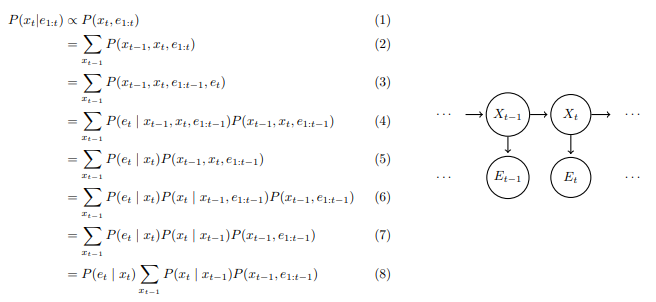
\includegraphics[scale=0.6]{figs/hmmderiv.png}\\
    \ifsol
    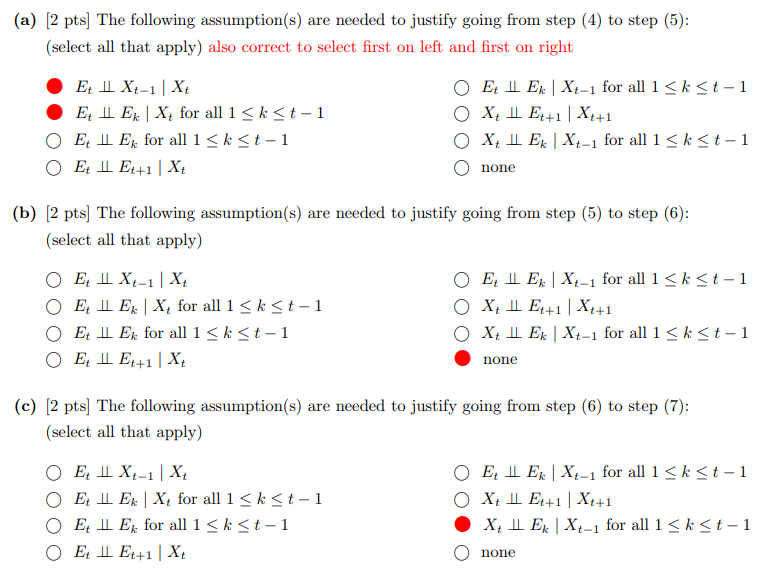
\includegraphics[width=\textwidth]{figs/hmmindepsol.png}\\
    \else
    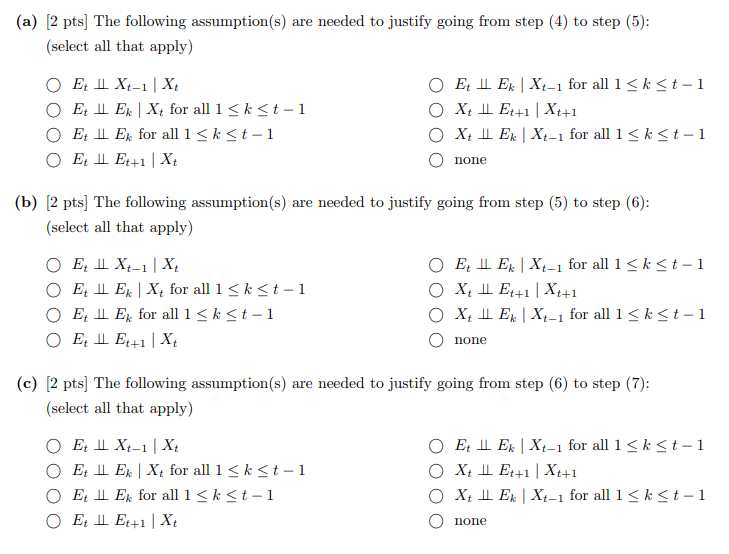
\includegraphics[width=0.9\textwidth]{figs/hmmindep.png}\\
    \fi

    \newpage
    \noindent \textbf{Problem 4:} Consider a Markov Model with a binary state $X$ (i.e., $X_t$ is either $0$ or $1$). The transition probabilities are given as follows:\\
    {\begin{center}
    \large
    \begin{tabular}{|c|c|c|}
    \hline
    \normalsize $X_t$ & \normalsize $X_{t+1}$ & \normalsize $P(X_{t+1} \mid X_t)$ \\ \hline
    \normalsize 0 & \normalsize 0 & \normalsize 0.9 \\ \hline
    \normalsize 0 & \normalsize 1 & \normalsize 0.1 \\ \hline
    \normalsize 1 & \normalsize 0 & \normalsize 0.5 \\ \hline
    \normalsize 1 & \normalsize 1 & \normalsize 0.5 \\ \hline
    \end{tabular}
    \end{center}}\\
    
    \begin{enumerate}{a) }
        \item \quad The prior belief distribution over the initial state $X_0$ is uniform, i.e., $P(X_0 = 0) = P(X_0 = 1) = 0.5$. After one timestep, what is the new belief distribution, $P(X_1)$?\\
        \begin{tabular}{|c|c|}
        \hline
        \normalsize $X_1$ & \normalsize $P(X_1)$ \\ \hline
        \normalsize 0 & \normalsize \ifsol {\color{blue} 0.7} \fi \\ \hline
        \normalsize 1 & \normalsize \ifsol {\color{blue} 0.3} \fi \\ \hline
        \end{tabular}\\
        \ifsol {\color{blue}
          The prior of $X_0$ is uniform, so the next step belief is the transition distribution from $X_0$:\\
          $p(X_1 = 0) = p(X_0 = 0)p(X_1 = 0|X_0 = 0) + p(X_0 = 1)p(X_1 = 0|X_0 = 1) =
          .5(.9) + .5(.5) = .7$.\\
          $p(X_1 = 1) = p(X_0 = 0)p(X_1 = 1|X_0 = 0) + p(X_0 = 1)p(X_1 = 1|X_0 = 1) =
          .5(.1) + .5(.5) = .3$.\\}
        \else
            \bigskip
        \fi
        \end{enumerate}
        
        Now, we incorporate sensor readings. The sensor model is parameterized by a number $\beta \in \left[0, 1\right]$:
    
        \begin{center}
        \large
        \begin{tabular}{|c|c|c|}
        \hline
        \normalsize $X_t$ & \normalsize $E_t$ & \normalsize $P(E_t \mid X_t)$ \\ \hline
        \normalsize 0 & \normalsize 0 & \normalsize $\beta$ \\ \hline
        \normalsize 0 & \normalsize 1 & \normalsize $(1-\beta)$ \\ \hline
        \normalsize 1 & \normalsize 0 & \normalsize $(1-\beta)$ \\ \hline
        \normalsize 1 & \normalsize 1 & \normalsize $\beta$ \\ \hline
        \end{tabular}
        \end{center}
        
        \begin{enumerate}{b)}
        \item \quad At $t=1$, we get the first sensor reading, $E_1 = 0$. Use your answer from part (a) to compute $P(X_1 = 0 \mid E_1 = 0)$. Leave your answer in terms of $\beta$. \\
        
        \ifsol {\color{blue}
        \begin{align*}
        p(X_1 = 0 | E_1 = 0) &= \frac{p(E_1 = 0 | X_1 = 0)p(X_1 = 0)}{\sum_x p(E_1 = 0 | X_1 = x)p(X_1 = x)} \\
        &= \frac{\beta(0.7)}{\beta(0.7) + (1-\beta)(0.3)} \\
        \end{align*}}
        \else
            \bigskip
            \bigskip
            \bigskip
            \bigskip
        \fi
        
        \item \quad For what range of values of $\beta$ will a sensor reading $E_1 = 0$ increase our belief that $X_1 = 0$? That is, what is the range of $\beta$ for which $P(X_1=0 \mid E_1=0) > P(X_1 = 0)$? \\
        
        \ifsol {\color{blue}
        $\beta \in \left(0.5, 1\right]$. Intuitively, observing $E_1 = 0$ will only increase the belief that $X_1 = 0$ if $E_1 = 0$ is more likely under $X_1 = 0$ than not. Note that $\beta > 0.5$; $\beta = 0.5$ is uninformative since the conditional distribution is uniform. This can be verified algebraically by setting $p(X_1 = 0) = p(X_1 = 0 | E_1 = 0)$ and solving for $\beta$.}
        \else
            \bigskip
            \bigskip
            \bigskip
            \bigskip
        \fi
    
    \end{enumerate}
%%%%%%%%%%%%%%%%%%%%%%%%%%%%%%%%%%%%%%%%%%%%%%%%%%%%%%%%%%%%%%%%%%%%%%%%%
%%%%%%%%%%%%%%%%%%%%%%%%%%%%%%%%%%%%%%%%%%%%%%%%%%%%%%%%%%%%%%%%%%%%%%%%%
\section{Bayes' Nets}
    \textbf{Problem 1:} Consider a Bayes Net with the following graph:\\
    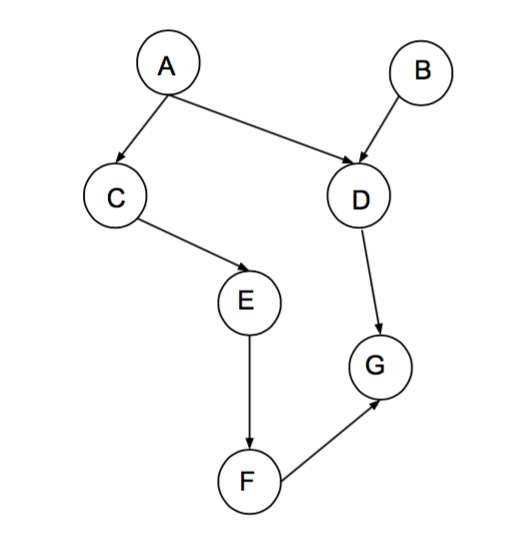
\includegraphics[scale=0.65]{figs/net1.png}\\
    Which of the following are guaranteed to be true without making any additional conditional independence assumptions, other than those implied by the graph? (Cirlce all true statements)
    \begin{itemize}
        \item \ifsol {\color{blue} $P(A|C,E)=P(A|C)$}
              \else $P(A|C,E)=P(A|C)$
              \fi
        \item $P(A,E|G)=P(A|G) \cdot P(E|G)$
        \item $P(A|B,G)=P(A|G)$
        \item \ifsol {\color{blue} $P(A|B=b)=P(A)$}
              \else $P(A|B=b)=P(A)$
              \fi
        \item \ifsol {\color{blue} $P(A,B|F)=P(A|F) \cdot P(B|F)$}
              \else $P(A,B|F)=P(A|F) \cdot P(B|F)$
              \fi
        \item $P(E,G|D)=P(E|D) \cdot P(G|D)$
    \end{itemize}

    \noindent \textbf{Problem 2:} Now consider a Bayes Net with the following graph:\\
    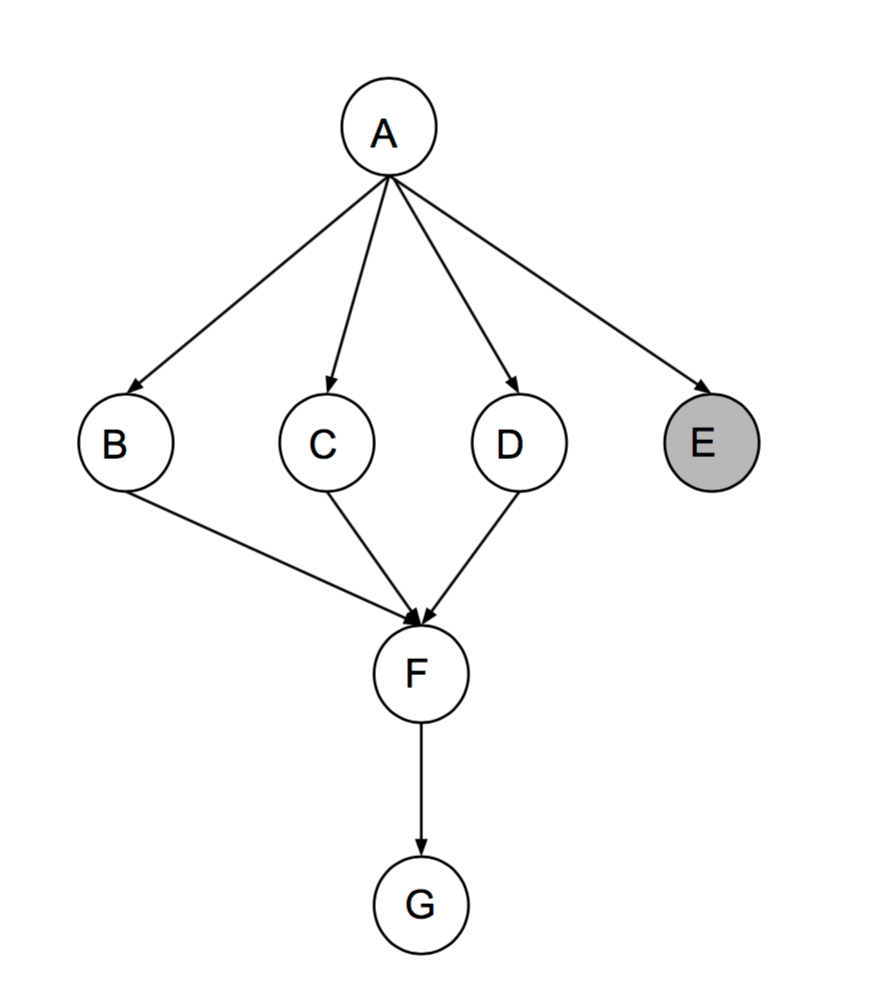
\includegraphics[scale=0.4]{figs/net2.png}\\
    The factors associated with the Bayes Net are $P(A), P(B | A), P(C | A), P(D | A), P(E | A), P(F | B,C,D)$ and $P (G | F )$. We will consider variable elimination to answer the query $P (G | +e)$.
    \begin{enumerate}[a)]
        \item Suppose the first variable we eliminate is A. Provide an expression for the resulting factor as a function of the original factors.\\
        \ifsol {\color{blue} $f_1(B,C,D,+e) =  \sum_a P(a)P(B | a)P(C | a)P(D | a)P(+e | a)$} \bigskip 
        \else \bigskip \bigskip \bigskip
        \fi
        
        \item Instead suppose the first variable we eliminate is B. Provide an expression for the resulting factor as a function of the original factors.\\
        \ifsol {\color{blue} $f_2(A,F,C,D) =  \sum_b P(b | A)P(F | b,C,D)$} \bigskip
        \else \bigskip \bigskip \bigskip
        \fi
        
        \item Instead suppose the first variable we eliminate is F. Provide an expression for the resulting factor as a function of the original factors.\\
        \ifsol {\color{blue} $f_3(B,C,D,G) =  \sum_f P(f | B,C,D)P(G | f)$} \bigskip 
        \else \bigskip \bigskip \bigskip
        \fi
        
        \item Instead suppose we eliminated the variables A, B, C, D, F in that order, and the single remaining factor is $f(+e,G)$. How do we obtain $P(G | +e)$ from this remaining factor? (Your answer should be in the form of an equation.)\\
        \ifsol {\color{blue} $P (G | +e) = \frac{f(+e, G)}{\sum_g f(+e, g)}$} \bigskip
        \else \bigskip \bigskip \bigskip
        \fi
    \end{enumerate}
    \textbf{Problem 3:}  Suppose that a patient can have a symptom (S) that can be caused by two different diseases (A and B). It is known that the variation of gene G plays a big role in the manifestation of disease A. The Bayes’ Net and corresponding conditional probability tables for this situation are shown below. For each part, you may leave your answer as an arithmetic expression.\\
    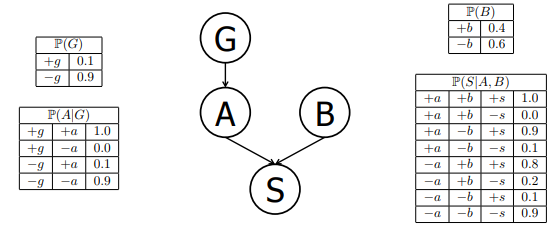
\includegraphics[scale=0.75]{figs/net3.png}\\
    \begin{enumerate}[a)]
        \item  Compute the following entry from the joint distribution: $P(+g, +a, +b, +s) =$\\
        \ifsol {\color{blue} $P(+g)P(+a| + g)P(+b)P(+s| + b, +a) = (0.1)(1.0)(0.4)(1.0) = 0.04$} \bigskip 
        \else \bigskip \bigskip \bigskip
        \fi
        
        \item  What is the probability that a patient has disease A?\\
        \ifsol {\color{blue} $P(+a) = P(+a| + g)P(+g) + P(+a| − g)P(−g) = (1.0)(0.1) + (0.1)(0.9) = 0.19$} \bigskip 
        \else \bigskip \bigskip \bigskip
        \fi
        
        \item  What is the probability that a patient has disease A given that they have disease B?\\
        \ifsol {\color{blue} $P(+a| + b) = P(+a) = 0.19.$ The first equality holds true as we have $A \independent B$, which can be inferred from the graph of the Bayes’ net.} \bigskip 
        \else \bigskip \bigskip \bigskip
        \fi
        
        \item What is the probability that a patient has the disease carrying gene variation G given that they have disease A? \\
        \ifsol {\color{blue} $P(+g| + a) = \frac{P(+g)P(+a|+g)}{P(+g)P(+a|+g)+P(−g)P(+a|−g)} = \frac{(0.1)(1.0)}{(0.1)(1.0)+(0.9)(0.1)} = \frac{0.1}{0.1+0.09} = 0.5263.$} \bigskip 
        \else \bigskip \bigskip \bigskip
        \fi
        
        \item What is the probability that a patient has the disease carrying gene variation G given that they have disease B?\\
        \ifsol {\color{blue} $P(+g| + b) = P(+g) = 0.1$ The first equality holds true as we have $G \independent B$, which can be inferred from the graph of the Bayes’ net.} \bigskip 
        \else \bigskip \bigskip \bigskip
        \fi
    \end{enumerate}
    
    \newpage
    \textbf{Problem 4:} Assume the following Bayes net, and the corresponding distributions over the variables in the Bayes net:\\
    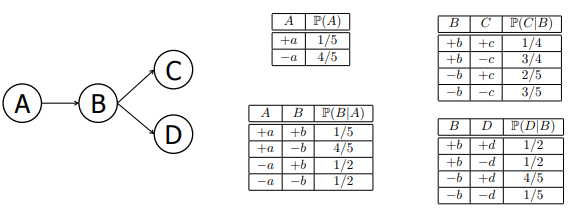
\includegraphics[scale=0.75]{figs/net4.png}\\
    \begin{enumerate}[a)]
        \item Your task is now to estimate $P(+b| −a, −c, −d)$ using rejection sampling. Below are some samples that have been produced by prior sampling (that is, the rejection stage in rejection sampling hasn’t happened yet). Cross out the samples that would be rejected by rejection sampling:\\
        \ifsol 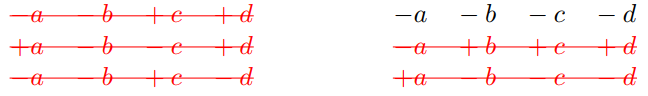
\includegraphics[scale=0.4]{figs/samplessol.png}\\
        \else 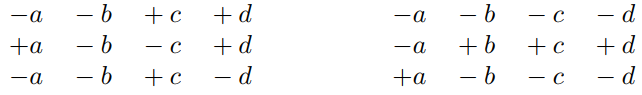
\includegraphics[scale=0.4]{figs/samples.png}\\
        \fi
        
        \item Using those samples, what value would you estimate for P(+b| − a, −c, −d) using rejection sampling?\\
        \ifsol {\color{blue} $0$} \bigskip
        \else \bigskip \bigskip
        \fi
        
        \item Using the following three samples (which were generated using likelihood weighting), estimate $P(+b | −a, −c, −d)$ using likelihood weighting, or state why it cannot be computed.\\
        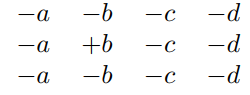
\includegraphics[scale=0.4]{figs/samples2.png}\\
        \ifsol {\color{blue} We compute the weights of each solution, which are the product of the probabilities of the evidence variables conditioned on their parents.
        $$w1 = w3 = P(−a)P(−c | −b)P(−d | −b) = 4/5 ∗ 3/5 ∗ 1/5 = 12/125$$
        $$w2 = P(−a)P(−c | +b)P(−d | +b) = 4/5 ∗ 3/4 ∗ 1/2 = 12/40$$
        so normalizing, we have $(w2)/(w2 + w1 + w3) = \frac{12/40}{12/40+12/125+12/125} = 25/41 ≈ 0.609756$.}
        \else \bigskip \bigskip \bigskip \clearpage
        \fi
    \end{enumerate}
%%%%%%%%%%%%%%%%%%%%%%%%%%%%%%%%%%%%%%%%%%%%%%%%%%%%%%%%%%%%%%%%%%%%%%%%%
%%%%%%%%%%%%%%%%%%%%%%%%%%%%%%%%%%%%%%%%%%%%%%%%%%%%%%%%%%%%%%%%%%%%%%%%%
\section{ML}
    \textbf{Problem 1:} \\
    For each of the following algorithms, describe how to evaluate whether $k$ is too small:
    \begin{itemize}
        \item k-means?
        \ifsol 
        {\color{blue}
        In k-means, $k$ determines the number of cluster centroids. If $k$ is too small, there may be a lot of internal structure that is assigned to a single cluster. As a result, there may be high "clustering error" (average distance from points to the cluster centroids) in comparison to slightly larger $k$.
        }
        \else \bigskip \bigskip \bigskip \bigskip \bigskip \bigskip
        \fi
        \bigskip
        
        \item k-NN?
        \ifsol 
        {\color{blue}
        In k-NN, $k$ determines the number of neighbors used to classify a new point. If $k$ is too small, the decision boundary between classes will be very rough/wobbly, and there may be higher error near the decision boundary relative to larger $k$.
        }
        \else \bigskip \bigskip \bigskip \bigskip \bigskip \bigskip
        \fi
    \end{itemize}
    
    \noindent \textbf{Problem 2:}\\
    
    \noindent Consider the following labeled data, along with four new points A, B, C, and D: \\
    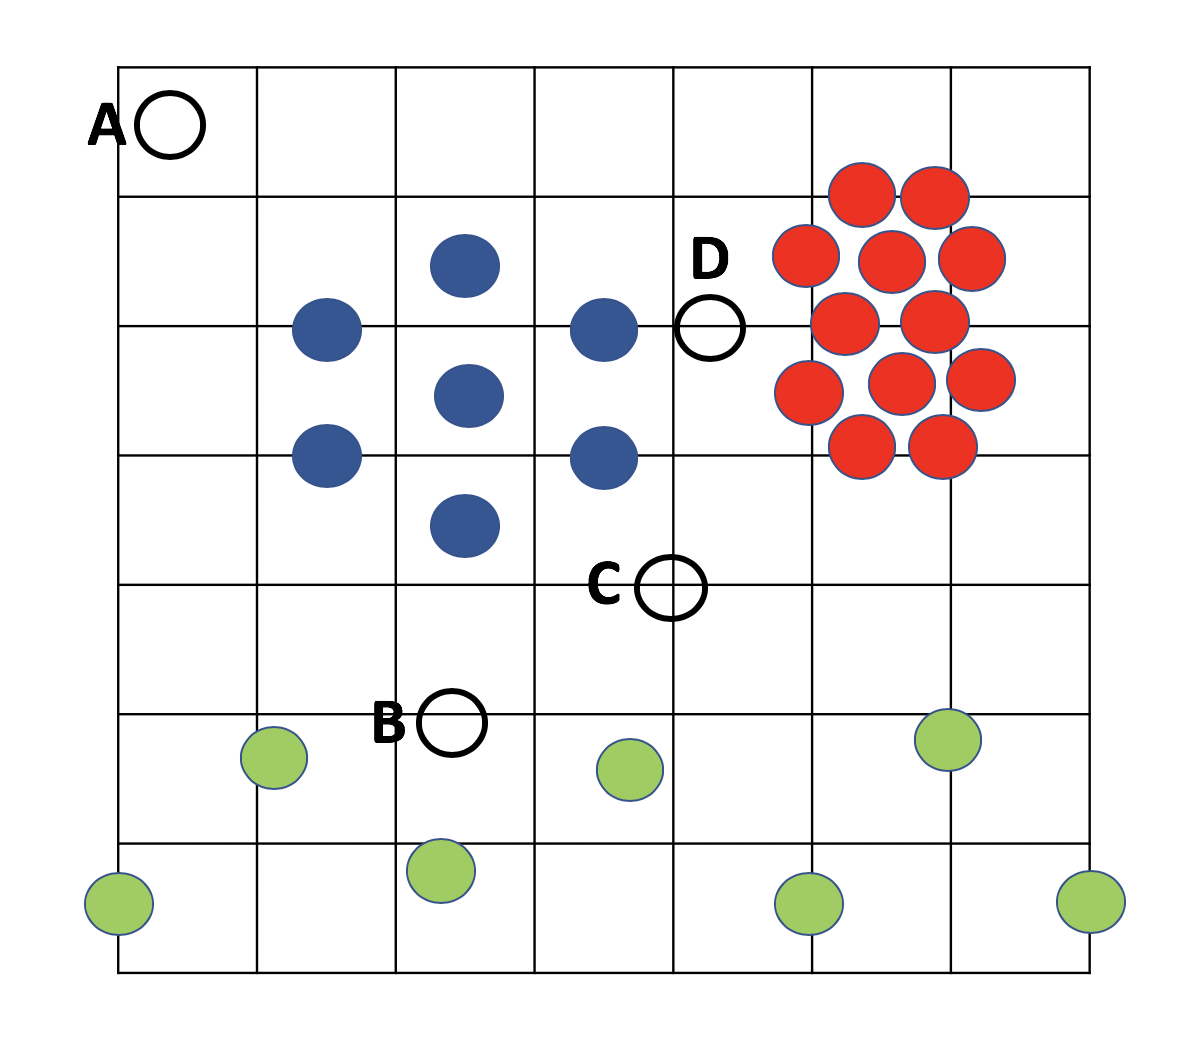
\includegraphics[scale=0.5]{figs/knn.png}
    
    \noindent What labels would be assigned to points A, B, C, and D if $k = 1$? \\
    \ifsol {\color{blue} A is blue, B is green, C is blue, D is blue.}
    \else \bigskip \bigskip \bigskip \bigskip \bigskip
    \fi
    \bigskip
    
    \noindent What labels would be assigned to points A, B, C, and D if $k = 4$? \\
    \ifsol {\color{blue} A is blue, B is green, C is blue, D is red.}
    \else \bigskip \bigskip \bigskip \bigskip \bigskip \bigskip
    \fi
    \bigskip
    
    \noindent \textbf{Problem 3:}\\
    
    \noindent You are a turnip farmer, and after a few years of tumultuous harvests, you decide to take a quantitative approach to agriculture. You decide to model your annual turnip yield (y) as a linear function of a single variable: the amount of rainfall in the previous year (x). So, after normalization, you have the following data points:
    \begin{table}[ht]
    	\center
    	\begin{tabular}{|c|c|}
    	\hline
    	turnip yield (y) & rainfall (x) \\
    	\hline
    	24 & 10 \\
    	\hline
    	33 & 14 \\
    	\hline
    	34 & 12 \\
    	\hline
    	\end{tabular}
    \end{table} \\
    Your are looking for a parameter $\theta$, and your model is $h_{\theta}(x) = \theta x$.
    \begin{enumerate}
        \item Suppose you are using a quadratic loss function ($L(h_{\theta}(x), y) = (h_{\theta}(x) - y)^2$), and you can choose $\theta$ to be equal to either 0, 1, 2, 3, or 4. Which is the best option for your data? \\
        \ifsol 
        {\color{blue} \noindent Looking at the relationship between $x$ and $y$, we can see that $\theta = 2$ would consistently underestimate $x$, and $\theta = 3$ would consistently overestimate $y$. Therefore, one of these is the best option out of the choices we are given. Since the goal of regression is to minimize the chosen loss function, we can calculate the quadratic loss for both of these values of $\theta$: \\
        
        If $\theta = 2$, then the total sum of squared errors is $(24 - 20)^2 + (33 - 28)^2 + (34 - 24)^2 = 4^2 + 5^2 + 10^2 = 141$. \\
        If $\theta = 3$, then the total sum of squared errors is $(24 - 30)^2 + (33 - 42)^2 + (34 - 36)^2 = 6^2 + 9^2 + 2^2 = 121$. \\
        
        Therefore, $\theta = 3$ is the best choice.
        }
        \else \bigskip \bigskip \bigskip \bigskip \bigskip
        \fi
        \bigskip
        
        \item Suppose you are using an $L_1$ loss function ($L(h_{\theta}(x), y) = |h_{\theta}(x) - y|$), and you can choose $\theta$ to be equal to either 0, 1, 2, or 3. Which is the best option for your data? \\
        \ifsol 
        {\color{blue} \noindent Similarly to the logic above, we can compare $\theta = 2$ and $\theta = 3$ by calculating the absolute loss for both of these values of $\theta$: \\
        
        If $\theta = 2$, then the total sum of absolute errors is $|24 - 20| + |33 - 28| + |34 - 24| = 4 + 5 + 10 = 19$. \\
        If $\theta = 3$, then the total sum of absolute errors is $|24 - 30| + |33 - 42| + |34 - 36| = 6 + 9 + 2 = 17$. \\
        
        Therefore, $\theta = 3$ is still the best choice.
        }
        \else \bigskip \bigskip \bigskip \bigskip \bigskip
        \fi
        \bigskip
    \end{enumerate}
    
    \noindent \textbf{Problem 4:}\\
    A few years later, you are a very successful farmer due to your skillful use of regression. Now, you farm not only turnips, but a large variety of vegetables; in fact, you decide which vegetables to plant each year using logistic regression:
    \[
    h_{\theta}(x) = \frac{1}{1 + e^{-\theta^T x}}
    \]
    Based on the total rainfall, normalized average temperature, and normalized market price (your input variable $x$), you decide whether the harvest will or will not be profitable (your output variable $y$, where $profitable$ = 1 and $not \;profitable$ = 0). Using a training dataset, you calculate the vector of optimal parameters:
    \[
    \theta = (-2, 1, 0.5)^T
    \]
    \begin{enumerate}
        \item This year, the total rainfall is 11, the normalized average temperature is 15, and the normalized current market price is -10. Does logistic regression predict that the harvest will or will not be profitable? \\
        \ifsol 
        {\color{blue} \noindent We can calculate the output of logistic regression by substituting new values into $h_{\theta}(x)$ above, and rounding to either 0 or 1. For this year, $-\theta^T x = -(-22 + 15 - 5) = 12$ so $h_{\theta}(x) = 1/(1 + e^{12})$ which is closer to 0 than 1. Therefore, the harvest is predicted to not be profitable.
        }
        \else \bigskip \bigskip \bigskip \bigskip \bigskip \bigskip
        \fi
        \bigskip
        
        \item In another year, the total rainfall is 11, the normalized average temperature is 15, and the normalized current market price is 24. Does logistic regression predict that the harvest will or will not be profitable? \\
        \ifsol 
        {\color{blue} \noindent Similarly to above, substitute: $-\theta^T x = -(-22 + 15 + 12) = -5$ so $h_{\theta}(x) = 1/(1 + e^{-5})$ which is closer to 1 than 0. Therefore, the harvest is predicted to be profitable.
        }
        \else \bigskip \bigskip \bigskip \bigskip \bigskip \bigskip
        \fi
        \bigskip
    \end{enumerate}
    
%%%%%%%%%%%%%%%%%%%%%%%%%%%%%%%%%%%%%%%%%%%%%%%%%%%%%%%%%%%%%%%%%%%%%%%%%
%%%%%%%%%%%%%%%%%%%%%%%%%%%%%%%%%%%%%%%%%%%%%%%%%%%%%%%%%%%%%%%%%%%%%%%%%
\newpage
\section{Game Theory}
    \noindent \textbf{Problem 1:} True or False: Every game with a Nash Equilibrium has a dominant strategy.\\
    \ifsol 
    {\color{blue} \noindent False. Many games have solutions that are mixed strategies -- for example (spoiler alert) the next two problems!}
    \else \bigskip \bigskip \bigskip
    \fi
    \bigskip
    
    \noindent \textbf{Problem 2:} This following is the matrix representation for the classic rock-paper-scissor game between a row player and a column player.\\
    \begin{table}[h]
    	\center
    	\begin{tabular}{|c|c|c|c|}
    		\hline
    	&Rock&Paper&Scissor\\
    		\hline
    		Rock& (0,0 )& (-1,1)& (1,-1)\\
    		\hline
    		Paper&(1, -1)& ( 0,0) & (-1,1)\\
    		\hline
    		Scissor&(-1,1)& ( 1, -1)& (0,0)\\
    		\hline
    	\end{tabular}
    \end{table}\\
    What is the Nash Equilibrium of this zero-sum game? Briefly explain why. \bigskip
    
    \ifsol 
    {\color{blue} \noindent One way to find the solution is to guess the equilibrium to be $(1/3,1/3,1/3)$ and then verify it. But it is hard to guess right in general so we will proceed by using Von Neumann's theorem (which we proved in class), which states that both player's Maximin strategy forms a Nash Equilibrium. \\
    
    \noindent We first compute the Maximin strategy for the row player. Let $p$ be the probability of playing \texttt{Rock} and $q$ be probability for \texttt{Paper}. Then the expected utility for the row player is: 
    	\begin{itemize}
    		\item when column player plays \texttt{Rock}: $q -(1-p-q)$
    		\item when column player plays \texttt{Paper}: $-p + (1-p-q)$
    		\item when column player plays \texttt{Scissor}: $p -q$ 
    	\end{itemize}
    Thus the Maximin strategy $(p^*,q^*, 1-p^* - q^*)$ solves the following optimization problem
    $$ \max_{p,q} \bigg[  \min{   \big\{ q -(1-p-q), -p + (1-p-q), p -q  \big\}  } \bigg]$$
    It is easy to verify that $p^* = q^* = 1/3$ is the optimal solution. Thus the Maximin strategy for the row player is $(1/3,1/3,1/3)$. By symmetry, the Maximin strategy for the column player is also $(1/3,1/3,1/3)$. 
    } 
    \else \bigskip \bigskip \bigskip \bigskip \bigskip \bigskip
    \fi
    \bigskip
    
    \noindent \textbf{Problem 3:} This following is the matrix representation for a zero-sum cop-robber game played between a cop (row player) and an robber (column player). The row player wants to catch the column player while the column player wants to avoid being caught. \\
    \begin{table}[h]
    	\center
    	\begin{tabular}{|c|c|c|c|}
    		\hline
    		&Location 1&Location 2\\
    		\hline
    Location 1 & (3,-3 )& (-2, 2)\\
    		\hline
    	Location 2&(-1, 1)& ( 2, -2) \\
    		\hline
    	\end{tabular}
    \end{table} \\
    What is the Nash Equilibrium of this zero-sum game? Briefly explain why. \bigskip
    
    \ifsol
    {\color{blue} \noindent Again we compute both player's Maximin strategies. For the row player (cop), let $p$ be the probability of visiting location 1. Then the expected utility for the row player is:
    \begin{itemize}
    	\item when column player visits location 1: $3p -(1-p)$
    	\item when column player visits location 2:  $-2p + 2(1-p)$
    \end{itemize}
    Thus the Maximin strategy $(p^*, 1-p^* )$ solves the following optimization problem
    $$ \max_{p} \bigg[  \min{   \big\{ 4p - 1, 2 - 4p \big\}  } \bigg]$$
    The optimal solution is $p^* = 3/8$. Thus the Maximin strategy for the row player is $(3/8,5/8)$. A similar procedure shows that the Maximin strategy for the column player is $(1/2,1/2)$.  
    } 
    \else \bigskip \bigskip \bigskip \bigskip \bigskip \bigskip
    \fi

\end{document}